\section{Suspension Commissioning Tasks}
In this section, we will describe what are some specific tasks needed to be done in order to achieve the aforementioned goals in Sec.~\ref{sec:goal}.
In next section, Sec.~\ref{sec:suspension_commissioning_baseline_methods}, we will describe some of the mathematical details on how to complete these tasks, and how to evaluate the performance of the suspensions.
In the section after the next, Sec.~\ref{sec:suspension_commissioning_advanced_methods}, we will review some methods that has been proposed but are not considered baseline.
Here, we encourage readers to choose and implement the methods themselves.
There's no best method.
And, we should emphasize that it's not important to use the same methods for all suspensions, but rather, to evaluate all suspensions using the same evaluation methods.
As long as we have a consistent evaluation scheme that ensures the requirements are met, that's it needs for KAGRA to work.

\subsection{List of tasks}
We will provide a list of tasks here in this section.
Further elaboration will be provided in the next.
These tasks are defined with the assumption that we have healthy hardware and we have sensors (and actuators) calibrated, and they are listed in order.

\begin{enumerate}
	\item (If not done already) Sensor noise measurement (and modeling).  \label{item:sensor_noise_measurement}
	\item (If not done already) Seismic noise measurement (and modeling). Use a worst-case spectrum, e.g. $90^\mathrm{th}$ percentile seismic noise in the winter season. \label{item:seismic_noise_measurement}
	\item Control Matrices
	\begin{enumerate}
		\item Install initial sensing matrices and actuation matrices from first principles.
		\item Modify sensing matrices or apply ``diagonalization''/``decoupling'' matrices so the readout is mapped to the desired basis (Cartesian coordinate + Euler angles).
		\item (Optional) Modify actuation matrices or apply ``diagonalization''/``decouping'' matrices so the actuations are also in the desired basis.
	\end{enumerate}
	\item Inter-calibration of sensors.
	\item Further sensor noise reduction tasks, e.g. sensor fusion and sensor correction. Redo step \ref{item:sensor_noise_measurement}.
	\item Transfer function (TF) measurements and modeling. Do for
	\begin{itemize}
		\item Diagonal actuation TFs in a stage-by-stage basis, \label{item:diagonal_tf}
		\item (Optional) Cross actuation TFs in a stage-by-stage basis, and \label{item:cross_tf}
		\item TFs from each displacement to optics/test mass (TM) degrees of freedom. \label{item:displacement_to_optics_tf}
	\end{itemize}
	\item From the highest stage (closest to the ground) to lowest stage, design the control filter and do the following \label{item:design_control_filter}
	\begin{enumerate}
		\item Predict the closed-loop displacement level and
		\item estimate the residual motion and displacement noise contribution to the optics using
		\begin{itemize}
			\item the seismic noise measurement/open-loop displacement levels from step \ref{item:seismic_noise_measurement} or step \ref{item:open_loop_displacement_levels},
			\item sensor noise measurement from step \ref{item:sensor_noise_measurement}, and
			\item the displacement-to-optics displacements transfer functions from step \ref{item:displacement_to_optics_tf}.
		\end{itemize} 
		\item Check stability using stability critera (Nyquist plot and stability margins.) and transfer functions from step \ref{item:diagonal_tf}.
		\item If any of the above failed, tune the control filter.
		\item Install the control filters and close the loop.
		\item Measure open-loop displacement levels of the next stage (Keep the controls at upper stage engaged.) and move on the next stage. \label{item:open_loop_displacement_levels}
		\item Repeat step \ref{item:design_control_filter} until all local control-loops at all stages are closed.
	\end{enumerate}
	\item Measure the residual motion using the sensors at the optics stage as an out-of-loop sensor (Do not engage the control-loops that use the optics' sensors). If this fails, find the problematic stage and redo all controllers starting from there.
	\item (If there exists an interferometer) Measure actuation to DARM transfer function and measure the displacement noise. If this fails, find the problematic stage and redo all controllers starting from there.
\end{enumerate}

\subsection{Further elaboration}
In order to achieve the displacement noise and residual motion requirements, as stated in Sec.~\ref{sec:displacement_noise_requirement} and Sec.~\ref{sec:residual_motion_requirement} respectively, we need to rely on a so-called control system.
Here we assume readers have basic understanding on control systems and are comfortable at working with frequency/Laplace domain quantities.
If not, please refer to introductory textbooks such as \cite{modern_control_engineering} and \cite{control_engineering}.

A suspension has a lot of degrees of freedom (DoFs).
KAGRA's control topology requires each DoF to be independent from each other.
Therefore each DoF can be thought as a single-input-single-output (SISO) system as shown in Fig.~\ref{fig:generalcontrolblockdiagram}.
\begin{figure}[!h]
	\centering
	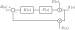
\includegraphics[width=75mm]{figures/general_control_block_diagram}
	\caption{Typical control block diagram of a single degree of freedom. $R(s)$: reference/setpoint, $D(s)$: external disturbance, $X(s)$: displacement, $N(s)$ sensing noise, $K(s)$: controller, $P(s)$: actuation transfer function.}
	\label{fig:generalcontrolblockdiagram}
\end{figure}
Now, we shall omit writing the bracket and assign capital letters to frequency/Laplace domain quantities and lower case letters for others.
Here, we define arbitrary functions $F(s)$ to be the Laplace transform of $f(t)$, where $s=\sigma+i\omega$ a complex number.
Typically, we analysis the functions by evaluating $s$ along the imaginary axis, i.e. frequency axis, so the functions we study here is closely related to the Fourier transform, and hence the amplitude spectral density, as we shall see later.
In Fig.~\ref{fig:generalcontrolblockdiagram}, $R$ is the setpoint, which is usually a static input at DC for coarse alignment purpose.
For most purposes in KAGRA's suspension, $R$ is considered to be $0$ at non-zero frequencies and therefore we will just mention it's existence but will not further discuss.
In the figure, $D$ is the external disturbance, that is, the open-loop spectrum of the displacement $X$\footnote{For a multiple stage suspension, $D$ is the displacement excited by motion at a higher stage.}.
$N$ is sensing noise, not sensor noise (we will properly define the meaning of $N$ later).
$K$ is the control filter, which is the filter that we need to design, and $P$ is the actuation transfer function of the suspension, which we need to model.

Here, the displacement reads
\begin{equation}
	X=\frac{1}{1+KP}\ D + \frac{KP}{1+KP}\ N.
	\label{eqn:X}
\end{equation}
From here, we shall define the proper definition of $N$ to be the limit of the displacement $X$ as the controller gain $K$ goes to infinity,
\begin{equation}
	N = \lim_{K\to\infty} X(K).
\end{equation}
So, it's not necessary sensor noise, but any residual signals present in the sensing readout\footnote{For example, the relative displacement sensors (LVDTs) at the preisolator of the Type-A and Type-B suspensions is coupled to ground motion, so the total sensing noise is a combination of the LVDT's intrinsic noise and seismic noise.}.
Continuing from Eqn.~\eqref{eqn:X}, the amplitude spectral density of $X$ is given by the quadrature sum of the filtered disturbance and sensing noise, i.e.
\begin{equation}
	X_\mathrm{ASD}(f) = \left[\left\lvert\frac{1}{1+KP}\right\rvert^2 D_\mathrm{ASD}^2(f) + \left\lvert\frac{KP}{1+KP}\right\rvert^2 N_\mathrm{ASD}^2(f)\right]^{\frac{1}{2}}.
\end{equation}
This is the quantity that we're interested in.
If this is the displacement of an upper stage, then we can estimate the displacement at the optics (TM) by
\begin{equation}
	X_\mathrm{ASD, TM}(f) = \left\lvert P_{X\to X_\mathrm{TM}}\right\rvert X_\mathrm{ASD}(f),
	\label{eqn:x_asd_tm}
\end{equation}
where $X_\mathrm{ASD, TM}(f)$ is the amplitude spectral density of the optics displacement $X_\mathrm{TM}$ and $P_{X\to X_\mathrm{TM}}$ is the transfer function from the displacement $X$ to the optics displacement $X_\mathrm{TM}$.

Once we can estimate the amplitude spectral density of the optics using Eqn.~\eqref{eqn:x_asd_tm}, we can tune 

\subsection{Control system preparatory tasks}
\subsubsection{Control matrices}
Now, before we can work with control systems, we need 
\subsection{Control tasks}

